\documentclass[a4paper]{article}
\usepackage[a4paper, total={6in, 9in}]{geometry}
\usepackage{amsmath}
\usepackage{csvsimple}
\usepackage{graphicx}
\usepackage{siunitx}
\usepackage{float}
\usepackage{subcaption}
\usepackage{blindtext}
\usepackage[hidelinks]{hyperref}
\usepackage[style=iso]{datetime2}

\graphicspath{ {./img/} }

\title{Laboration i Geometrisk Optik}

\author{Emil Babayev}
\date{\today}
\begin{document}
\begin{titlepage}
	\centering
	
\includegraphics[width=0.15\textwidth]{logo.png}\par\vspace{1cm}
	{\scshape\large Lunds Universitet \par}
	\vspace{1cm}
    {\scshape\large FAFF30 Våglära och optik\par}
	\vspace{1.5cm}
	{\huge\bfseries Laborationsrapport\\Geometrisk Optik\par}
	\vspace{2cm}
	{\Large Emil Babayev\par}
	\vfill
	Laborationshandledare\par
    David Gustavsson \par
    Rebecca Ahrling

    \vfill
    
	{\large \today \par}
\end{titlepage}

\section{Inledning}
\subsection{Introduktion och sammanfattning}
I denna laboration har två optiska komponenters egenskaper och karaktäristik undersökts. Under laborationen har prismor
och linser undersökts. Därutöver har kollimering och linjering diskuterats och beskrivits. Hela den experimentella delen har genomförts
digitalt i programmet Geometrical Optics Tool, skrivet av en tidigare student. Prismor och linser är optiska komponenter
som spelar en viktig roll i vår vardag, exempelvis i kameror, glasögon, luppar med mera. Därför finns det god motivation 
till att genomföra en laboration likt denna för att förstå optiska komponenters egenskaper.

Avståndet till ljuskällan, placering på den optiska axeln, rotation kring den optiska axeln och olika typer av avbildningsfel
har undersökts för linsen och kommer diskuteras i rapporten. Vad gäller prismor har man experimentellt försökt hitta minsta avlänkningsvinkel
för olika våglängder.

Sammanfattningsvis kan vi formulera en kort frågeställning: Hur beter sig linser i olika förhållanden, och hur kan man experimentellt beräkna minsta 
deviation(avlänkningsvinkel) för ett prisma?

Undersökningen har lett till följande slutsatser: Linser är känsliga optiska instrument som inte fokuserar rätt om vi avviker från optimala förhållanden,
och drabbas lätt av avbildningsfel. Prismat hade i vårt fall hade en minsta deviation på runt \ang{60}. 
\subsection{Introduktionsuppgifter}
För uppgift 1, se appendix A om kollimering och linjering. 
Uppgift 2 beskrivs här nedan.
Använder formlen för minimiavlänkning, ekvation \ref{eq: avl}\cite[p. 212]{vl}, där $n$ är brytningsindex i materialet, $\delta$ är avlänkningsvinkeln och 
$\alpha$ är vinkeln mellan de brytande ytorna i prismat.
\begin{equation}
    \label{eq: avl}
    n = \frac{sin(\frac{\delta +\alpha}{2})}{sin(\frac{\alpha}{2})}
\end{equation}
och löser ut $\delta$, som vi söker. Detta ger ekvation \ref{eq: avl2}:
\begin{equation}
    \label{eq: avl2}
    \delta = 2 arcsin(n sin\big(\frac{\alpha}{2}\big)) - \alpha
\end{equation}
Insättning av $n=1.57$ och $\alpha = \ang{60}$ ger $\delta = \ang{43.44}$.

\section{Teori}
\subsection{Divergens hos en stråle}
Divergensen hos en ljuskälla definieras som vinkeln hos ljuskonen som bildas när ljuset propagerar \cite{wiki}. Divergensvinkeln $\theta$ kan beräknas med ekvation \ref{eq: div}:
\begin{equation}
    \theta = 2 arctan\Big(\frac{d_1 - d_2}{2l}\Big)
    \label{eq: div}
\end{equation}
Sambandet kan härledas om man iakttar en del av ljuskonen som är långt borta från alla fokus och utför lite trigonometri. Se figur \ref{fig:divergens}. $d_1$ och $d_2$
är ljuskonens diameter i två punkter, och $l$ är avståndet där emellan.  
\begin{figure}[h!]
    \centering
    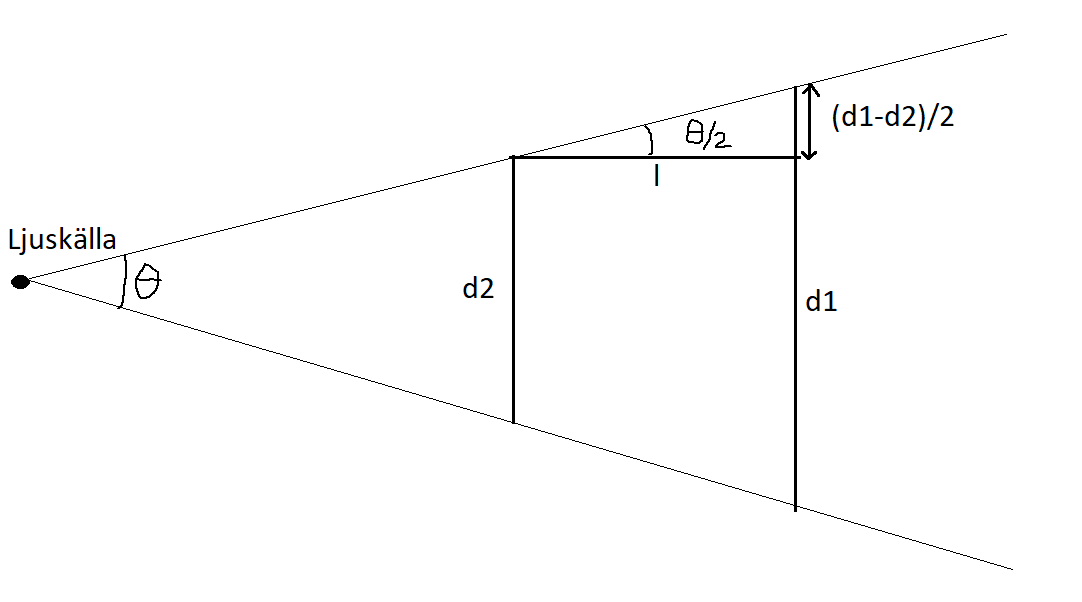
\includegraphics[width=0.6\textwidth]{divergens}
    \caption{Härledning av divergensvinkel}
    \label{fig:divergens}
\end{figure}
\pagebreak
\subsection{Optiska komponenter}
De optiska komponenter som används i laborationen är prismor och konvexa linser.
\subsubsection{Prismor}
Prismat är en komponent med platta genomskinliga ytor, där ljuset bryts då det propagerar. Vi tittar på triangulära prismor i denna laboration,
där varje gränsyta följer Snells brytningslag, ekvation \ref{eq:brytning}\cite[p.202]{vl}. $n$ brytningsindex. $\alpha$ infalls-/brytningsvinkel.
\begin{equation}
    n_1*sin(\alpha_1) = n_2*sin(\alpha_2)
    \label{eq:brytning}
\end{equation}
Varje gång en ljusstråle passerar igenom en gränsyta bryts det. I vårt fall bryts det mot normalen när det äntrar prismat, eftersom prismat är av glas och vi antar luft utanför.
När det sedan lämnar prismat bryts det bort från normalen. Detta resulterar i att ljuset böjs av en viss vinkel jämfört med den ursprungliga riktningen. Denna vinkel kallas
avlänkningsvinkeln, eller deviationen, som vi betecknar med $\delta$ . Den brytande kanten på prismat får också en egen vinkel, $\alpha$. Se figur \ref{fig:prism}.
\begin{figure}[h!]
    \centering
    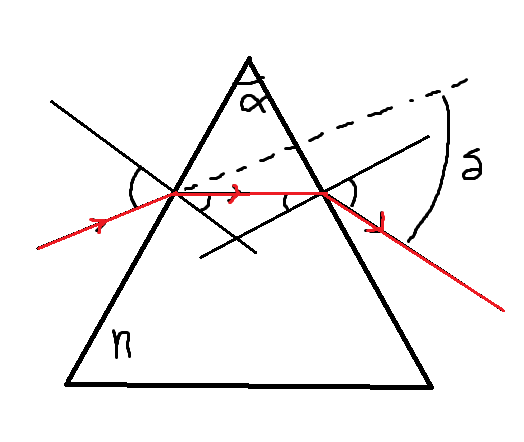
\includegraphics[width=0.5\textwidth]{prism.png}
    \caption{Principskiss av prisma. Strålgången är markerad i rött.}
    \label{fig:prism}
\end{figure}
Avlänkningsvinkeln blir minst då strålgången är symmetrisk kring prismat \cite[p.210-211]{vl}. Det finns en formel för minsta avlänkningsvinkel, ekvation \ref{eq:avlankning} \cite[p.212]{vl}.
\begin{equation}
    n = \frac{sin(\frac{\delta +\alpha}{2})}{sin(\frac{\alpha}{2})}
    \label{eq:avlankning}
\end{equation}

\subsubsection{Linser}
Linserna vi pratar om i laborationen är två sfäriska, sammanfogade gränsytor som buktar utåt (konvexa). Även i linser gäller 
Snells brytningslag. Med hjälp av linser kan strålar fokuseras. Punkten (reell eller virtuell) där alla strålar fokuseras
kallas brännpunkten. För tunna linser gäller (med vissa antaganden) Gauss linsformel, ekvation \ref{eq:gauss} \cite[p.230]{vl}. Beteckningar enligt
figur \ref{fig:lens}.
\begin{equation}
    \frac{1}{a} + \frac{1}{b} = \frac{1}{f}
    \label{eq:gauss}
\end{equation}
\begin{figure}[h!]
    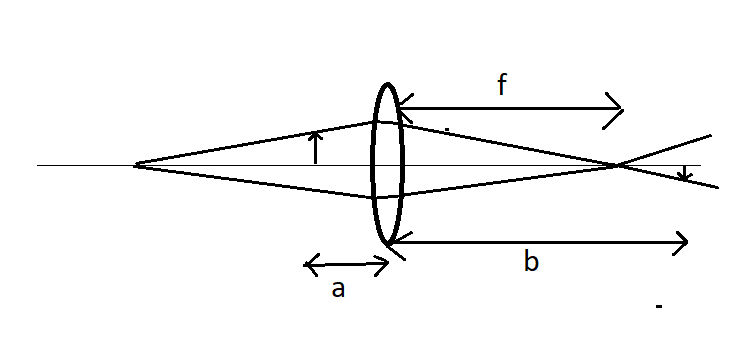
\includegraphics[height=0.3\textheight]{lens.png}
    \caption{Principskiss av en lins. Ett objekt avbildas på andra sidan, fast mindre.}
    \label{fig:lens}
\end{figure}
\subsection{Avbildningsfel}
I denna laboration diskuteras tre typer av avbildningsfel. Avbildningsfel skapar hinder vid design av optiska komponenter.
De tre typerna är:
\begin{itemize}
    \item Koma, där ljus som kommer in snett mot linsens optiska axel bryts olika mycket. Därmed skapas en utsmetad
    avbildning på andra sidan linsen \cite{ins}. Se figur \ref{fig:got}f.
    \item Sfärisk aberration, som beror på att ljus som når sfäriska gränsytor inte bryts på samma sätt i kanten av linsen som paraxiala strålar.
    Strålarna som når kanten får en kortare brännvidd \cite[p.238]{vl}. Se figur \ref{fig:got}g.
    \item Kromatisk aberration, som beror på att glas med samma brytningsindex inte bryter ljus med olika våglängd
    likadant. Varje våglängd får därmed en egen fokalpunkt och bilden blir ofokuserad  \cite[p.237]{vl}. Se figur \ref{fig:got}h.
\end{itemize}
\section{Material och metod}
Det fysiska materialet för denna laboration har endast varit en dator. Programvaran som tillhandahölls
av institution är Geometric Optics Tool för analys av optiska komponenter och MATLAB för dataanalys. 
Dessa program erbjöds av institutionen och därför fanns inte så mycket annat att välja på. För mätning
av vinklar på skärmen användes programmet MB-Ruler eftersom det var lättillgängligt och gratis.

Arbetssättet i Geometrical Optics Tool (hädanefter förkortat som GOT) liknade det det skulle gjort
i en verklig laborationssal. Uppställningen sattes upp enligt instruktioner i programmet, 
resultat iakttogs och sedan dokumenterades uppställningen genom att ta en skärmdump av akutell uppställning.

För att mäta avlänkningsvinkeln i prismat användes programmet MB-Ruler som är en digital linjal
som kan mäta vinklar och avstånd på skärmen.

I just denna laboration placerades en lins framför en divergent ljuskälla i GOT. Den flyttades och roterades och undersöktes.
Sedan placerades ett prisma ut som roterades för att mäta avlänkningsvinkel. 
\section{Resultat}
\subsection{Beräkning av divergens} \label{div}
Jag valde två punkter och avståndet $d_1 = 9.28$ l.e., $d_2 = 5.40$ l.e., $l = 7$ l.e.
Insättning i ekvation \ref{eq: div} gav en vinkel $\theta = \ang{31.28}$.

\subsection{Mätvärden från prismat}

\begin{table}[h]
    \begin{tabular}{|l|l|}
    \hline
    Infallsvinkel & Avlänkningsvinkel \\ \hline
    50.04         & 75.49             \\ \hline
    57.21         & 65.26             \\ \hline
    60.29         & 64.55             \\ \hline
    63.33         & 64.48             \\ \hline
    65.99         & 64.59             \\ \hline
    70.71         & 66.46             \\ \hline
    80.81         & 71.95             \\ \hline
    90            & 77.63             \\ \hline
    \end{tabular}
    \caption{Ljusets våglängd 555 nm. Alla mätvärden anges i grader.}
    \label{tb:555}
\end{table}

\begin{table}[h]
    \begin{tabular}{|l|l|}
    \hline
    Infallsvinkel & Avlänkningsvinkel \\ \hline
    45.98         & 90                \\ \hline
    50.25         & 62.88             \\ \hline
    60.04         & 59.69             \\ \hline
    60.42         & 59.27             \\ \hline
    65.44         & 60.27             \\ \hline
    70.36         & 61.89             \\ \hline
    80.74         & 67.70             \\ \hline
    89.65         & 75.45             \\ \hline
    \end{tabular}
    \caption{Ljusets våglängd 700 nm. Alla mätvärden anges i grader.}
    \label{tb:700}
\end{table}
\pagebreak
\subsection{Uppställningar från GOT}

\begin{figure}[h!]
    \begin{tabular}{cc}
    \subfloat[Lins långt ifrån källan]{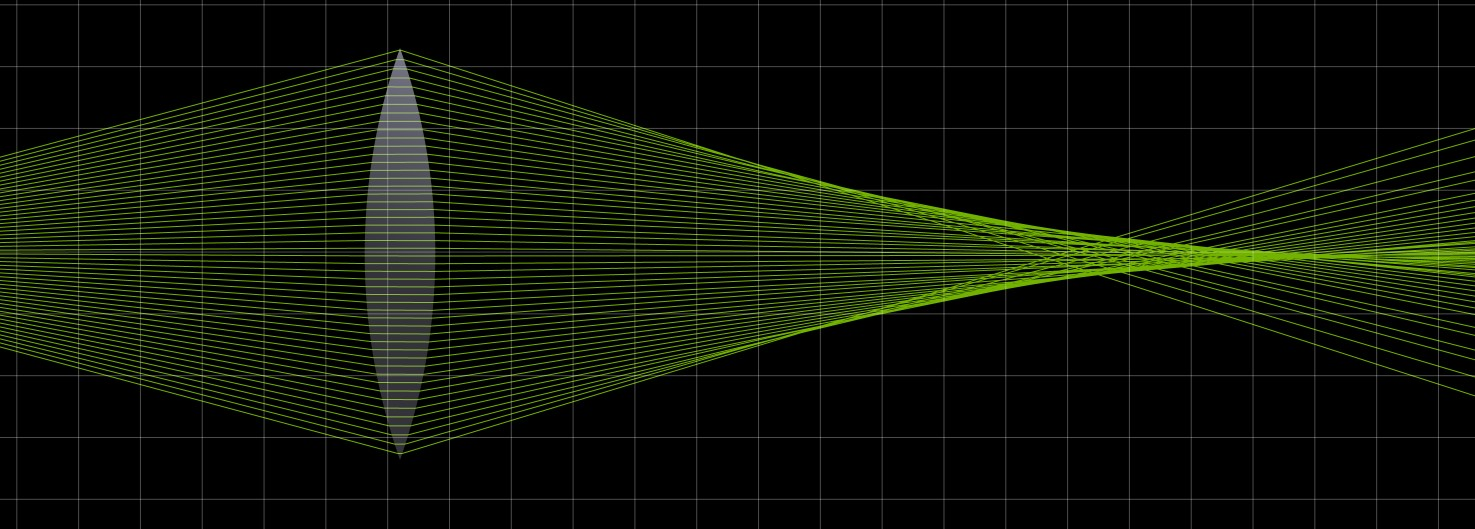
\includegraphics[width = 3in]{litenb.jpg}} &
    \subfloat[Lins nära källan]{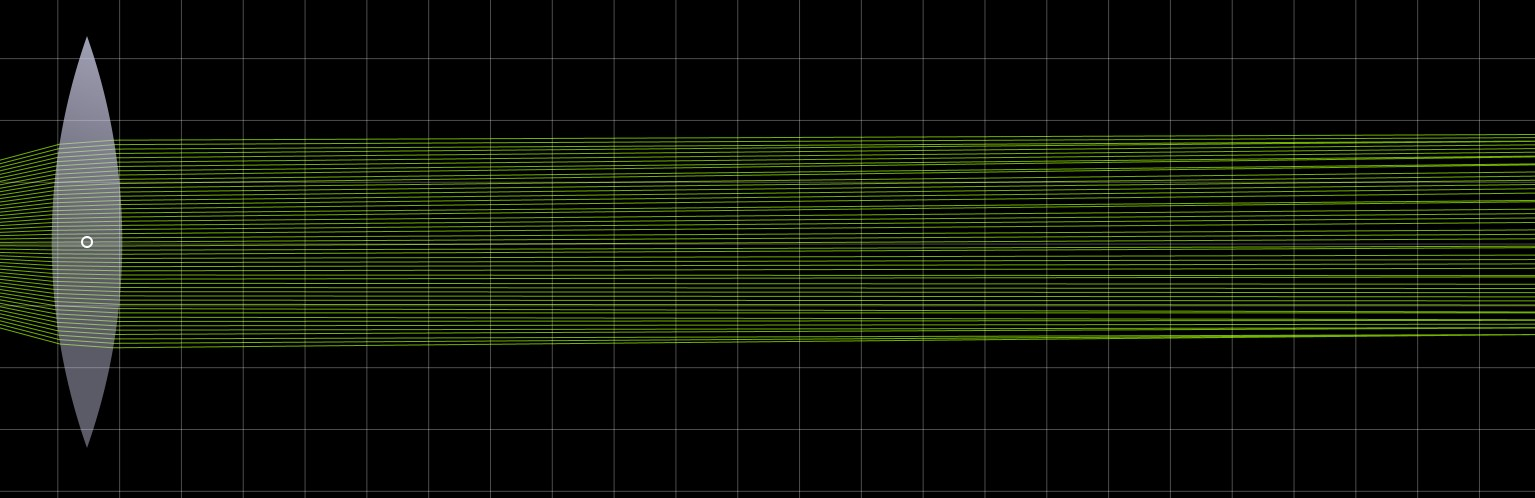
\includegraphics[width = 3in]{langb.jpg}}\\
    \subfloat[Sned lins]{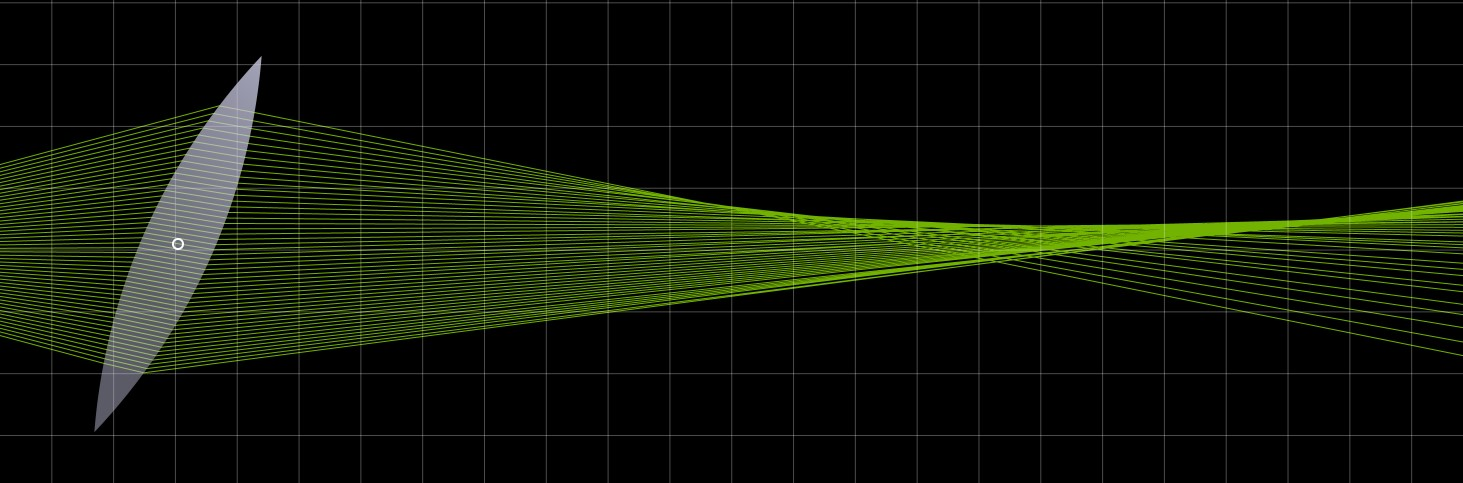
\includegraphics[width = 3in]{sned.jpg}} &
    \subfloat[Lins förskjuten i planet]{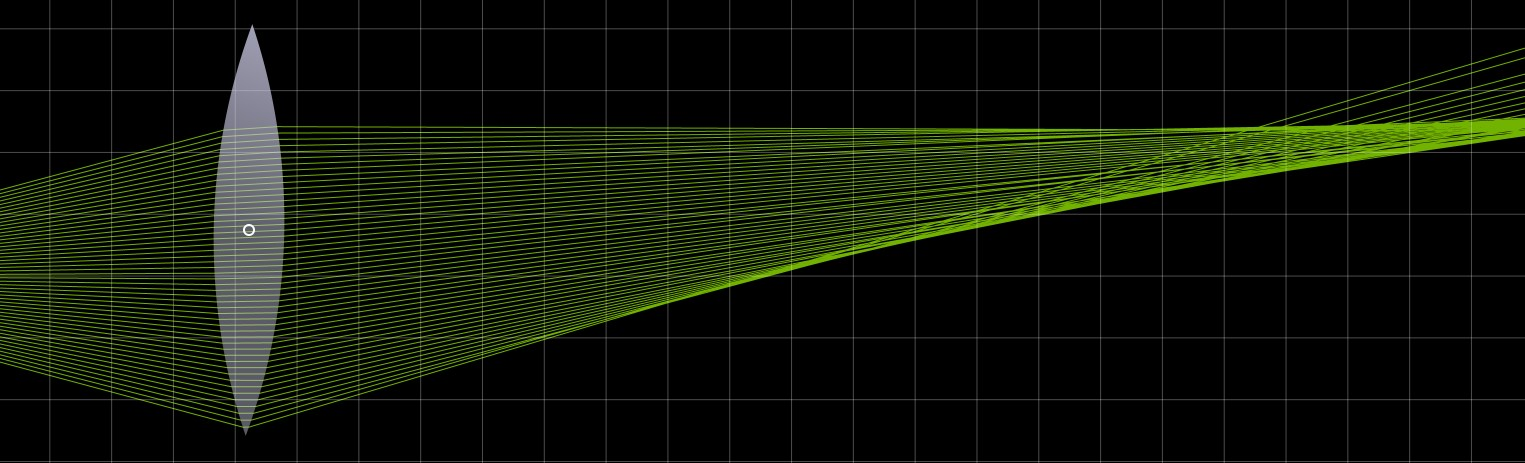
\includegraphics[width = 3in]{skev.jpg}}\\
    \subfloat[Ungefär samma avstånd till källan som brännpunkten.]{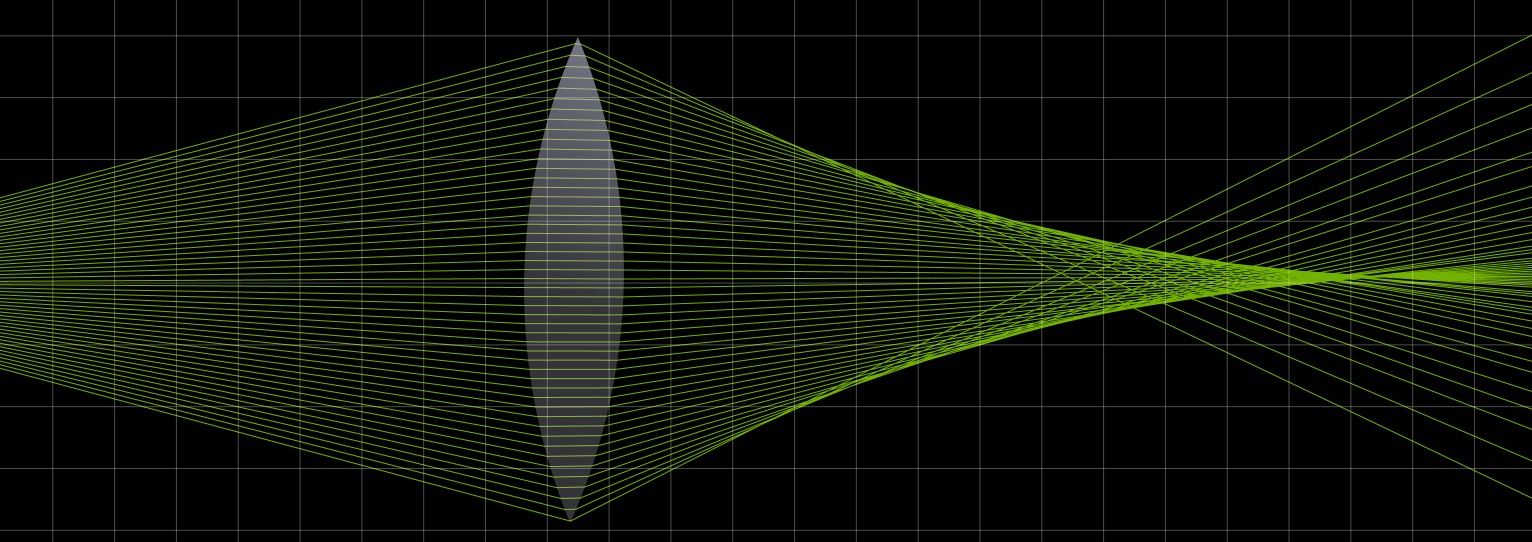
\includegraphics[width = 3in]{lika.jpg}} &
    \subfloat[Koma, ljuset kommer in snett och "smetas ut"]{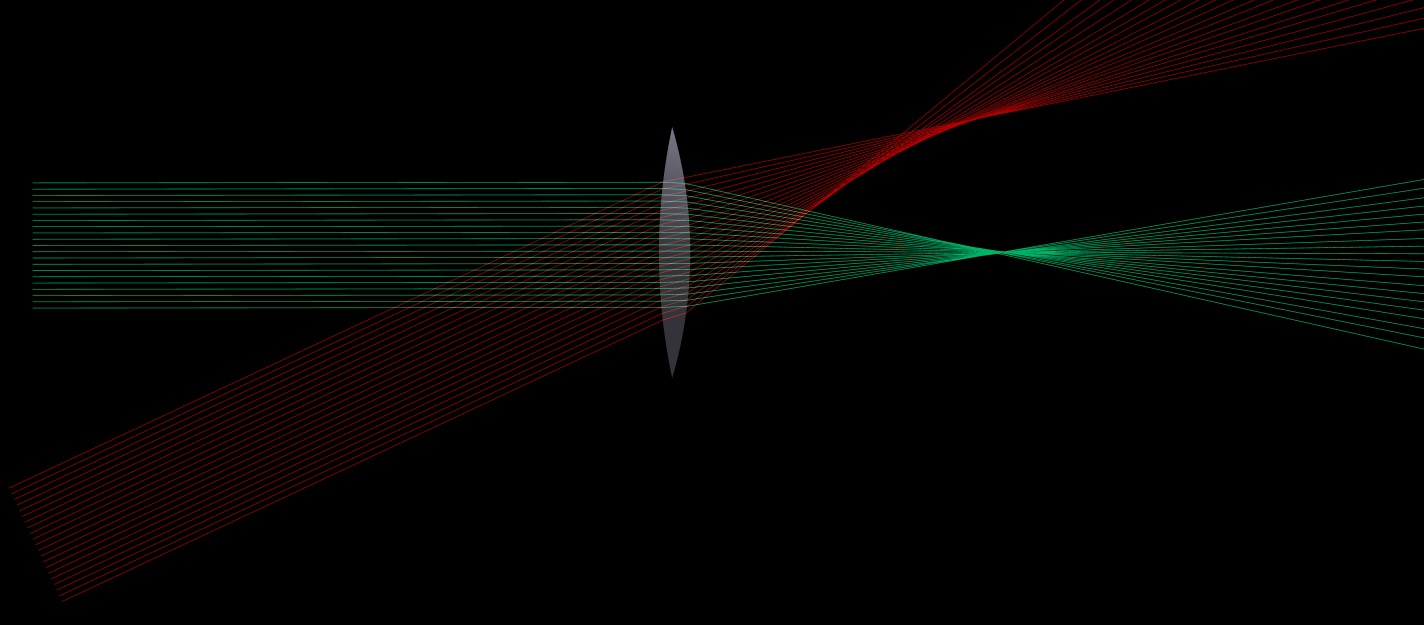
\includegraphics[width = 3in]{koma.jpg}}\\
    \subfloat[Sfärisk aberration, allt ljus fokuseras inte i brännpunkten.]{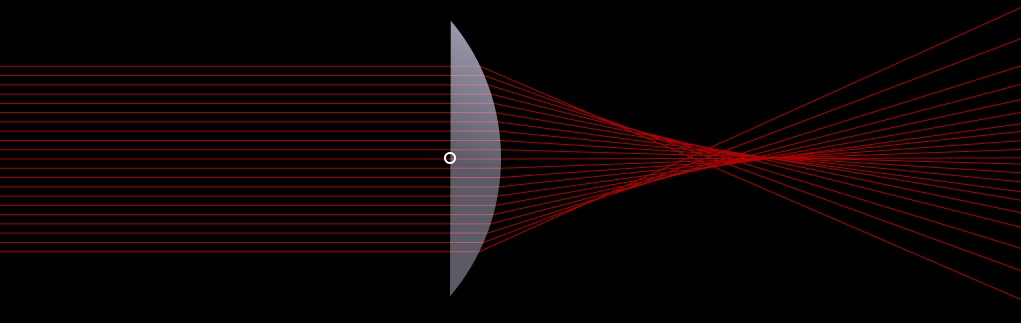
\includegraphics[width = 3in]{sphabherr.jpg}} &
    \subfloat[Kromatisk aberration, olika väglängder fokuseras på olika brännpunkter.]{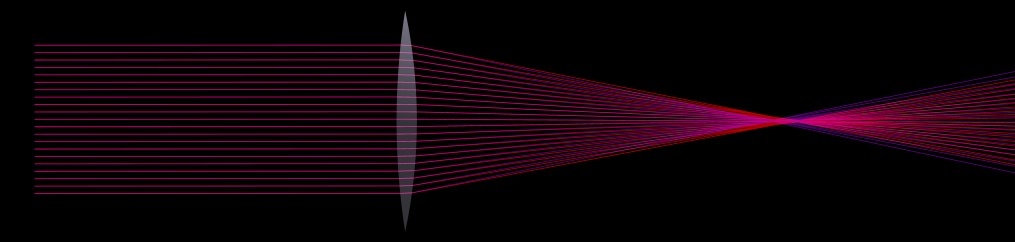
\includegraphics[width = 3in]{kromabherr.jpg}} \\
    \subfloat[Skarp brännpunkt]{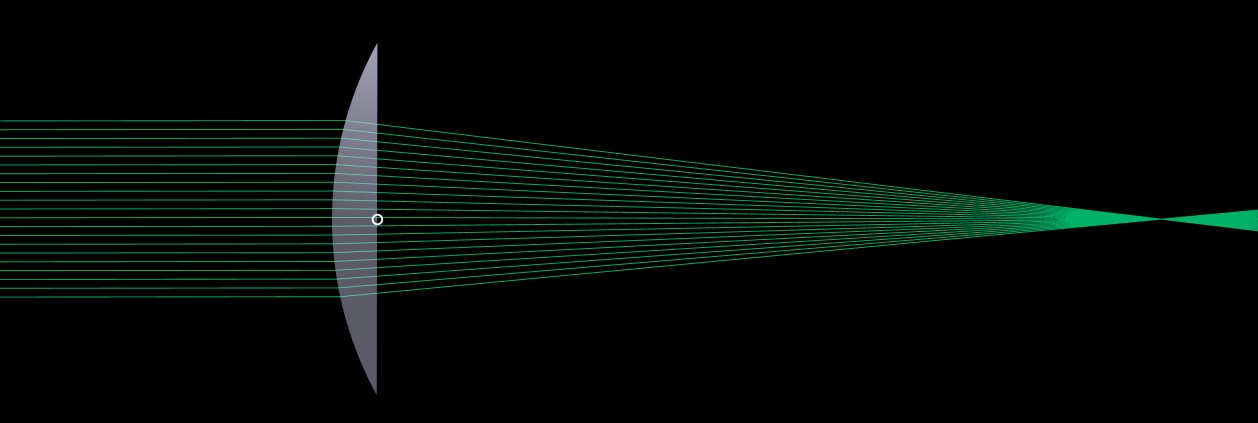
\includegraphics[width = 3in]{goodfocus.jpg}} &
    \subfloat[Oskarp brännpunkt]{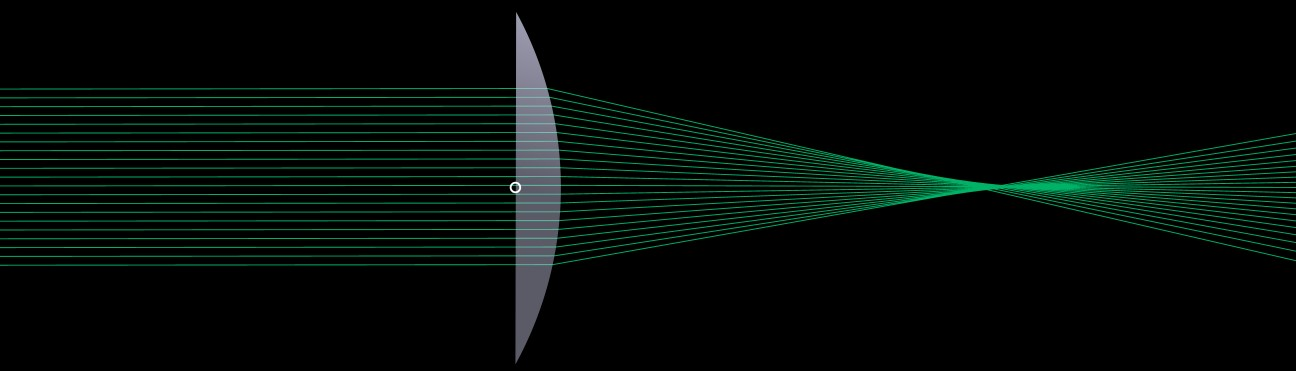
\includegraphics[width = 3in]{badfocus.jpg}} \\
    \subfloat[Totalreflektion i en rektangulär komponent.]{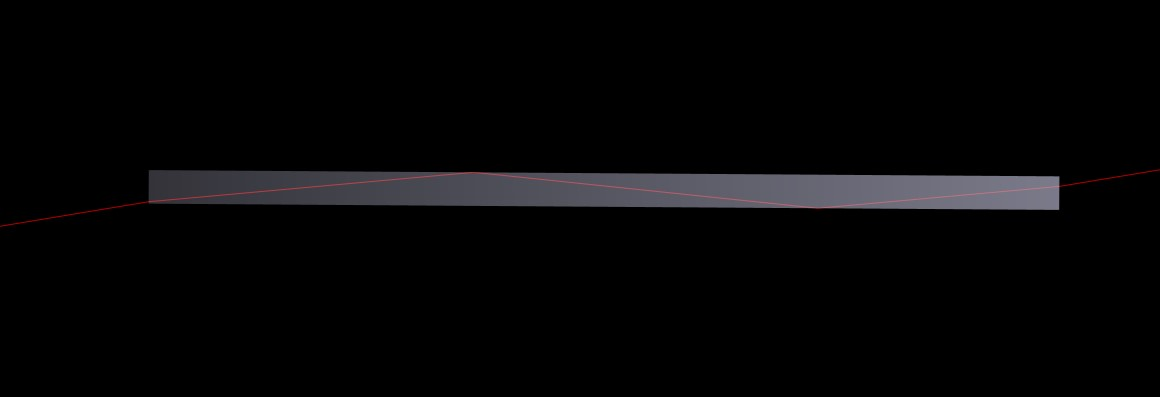
\includegraphics[width = 3in]{total.jpg}} 
    \end{tabular}
    \caption{De olika uppställningarna i GOT}
    \label{fig:got}
    \end{figure}

\pagebreak

\section{Diskussion och slutsatser}
\subsection{Linser}
Inledningsvis kan vi etablera att divergensvinkeln som beräknas i sektion \ref{div} är rimlig.

Efter noggrann undersökning kan man dra en del slutsatser om hur en lins beter sig. Det som kunde iakttas var att
ju närmare linsen placeras till ljuskällan, ju större blir brännvidden, för att till slut bli oändlig. Då får vi
parallella strålar från en divergent ljuskälla. Detta demonstreras i resultatet, figur \ref{fig:got}a. 
När vi istället placerar linsen långt ifrån ljusskällan får vi motsatt effekt, brännvidden minskar, och strålarna
fokuseras i en brännpunkt. Brännpunkten kommer närmare linsen ju längre bort linsen placeras från ljusskällan. Se figur \ref{fig:got}b.

Rotation och förflyttning av linsen gav liknande resultat. En rotation av linsen förskjöt bränn-
punkten uppåt eller nedåt, om än lite. Se figur \ref{fig:got}c. Samtidigt bryts inte alla strålar i samma plan och brännpunkten
blir "utsmetad". Med en roterad lins går det antagligen inte att få en fokuserad bild av hela objektet. Med en lins
som är förskjuten i samma plan (figur \ref{fig:got}d) flyttas brännpunkten upp eller ned mycket mer. Samtidigt blir
brännpunkten mycket mindre utsmetad, antagligen eftersom alla strålar bryts i ungefär samma plan. Min gissning är att
det borde gå att få en fokuserad bild om man endast förskjuter linsen i samma plan.

Sedan placerades linsen så att avståndet till ljuskällan var ungefär samma som avståndet till brännpunkten, figur \ref{fig:got}e.
För att ta reda på vad detta avstånd är, uttryckt i linsens brännvidd, användes Gauss linsformel, ekvation \ref{eq:gauss}. Det enda vi
känner till är att avståndet $a = b$ i formeln, och att båda dessa avstånd är en multipel av brännvidden $f$. Med dessa antaganden
kan vi då sätta $a = b = cf$ i $ \frac{1}{a} + \frac{1}{b} = \frac{1}{f}$. Löses ekvationen fås $c=2$ alltså $a=b=2f$. Avståndet mellan
lins och fokalpunkt är alltså två brännvidder. Resultatet är diskuterbart med tanke på att ekvation \ref{eq:gauss} egentligen endast gäller
för tunna linser och linsen som användes inte var tunn. Samtidigt känns det rimligt att avståndet är en heltalsmultipel. Däremot känns det
fel rent intuitivt med tanke på att avståndet mellan lins och brännpunkt borde vara definierat som just brännvidden, alltså att $c = 1$.

Sedan återskapades tre avbildningsfel med hjälp av GOT, sfärisk aberration, koma och kromatisk aberration. Resultatet från dessa undersökningar
återfinns i figurer \ref{fig:got}f-h. Det syns tydligt att ljusstrålarna böjs av mer när de propagerar genom linsens kant, jämfört med propagation
genom linsens mitt, den "tjockare" delen, alltså uppstår sfärisk aberration i figur \ref{fig:got}g. Samtidigt syns förskjutningen och defokuseringen
av fokalpunkten tydligt i figur \ref{fig:got}f, när ljuset kommer in snett mot den optiska axeln, där ett koma uppstår. Likaså syns det, om inte lika 
tydligt att brännpunkten förskjuts beroende på ljusets våglängd i figur \ref{fig:got}h, då kromatisk aberration uppstår.

Har man en plankonvex lins är det bättre att placera den konvexa sidan mot ljuskällan, jämför figurer \ref{fig:got}i och \ref{fig:got}j. Då motverkas
sfärisk aberration och fokalpunkten blir skarp. Anledningen till att sfärisk aberration motverkas skulle jag gissa på är att ljuset i detta fall bryts 
när det äntrar linsen, och endast en gång, vilket leder till att sfärisk aberration inte uppstår.

\subsection{Prismat}
Vad gäller prismat togs ett tiotal mätvärden, för två våglängder, $\lambda_1=\SI{555}{\nano\meter}$ och $\lambda_2=\SI{700}{\nano\meter}$.
Dessa återfinns i tabell \ref{tb:555} och \ref{tb:700}. Mätvärdena plottades i MATLAB och för att skapa en kontinuerlig avlänkningskurva
valde jag att anpassa tredjegradspolynom till mätdatan. Plotten och kurvorna syns i figur \ref{fig: plot}. Att göra denna anpassningen
fungerade bra för $\lambda_1$ men inte riktigt lika bra för $\lambda_2$. Antagligen hade jag bara tur i anpassningen. Med hjälp av dessa
anpassade kurvor sökte jag sedan minsta avlänkningsvinkel numeriskt och fick ut minsta deviation $\delta_1 = \ang{64.0680}$
för $\lambda_1$ och $\delta_2 = \ang{57.5861}$ för $\lambda_2$. Detta resultat kan diskuteras på två sätt: rimligheten hos resulatet och
rimligheten hos metoden som användes för att få fram resulatet. Vi börjar med det förstnämnda.

\begin{figure}[h]
    \centering
    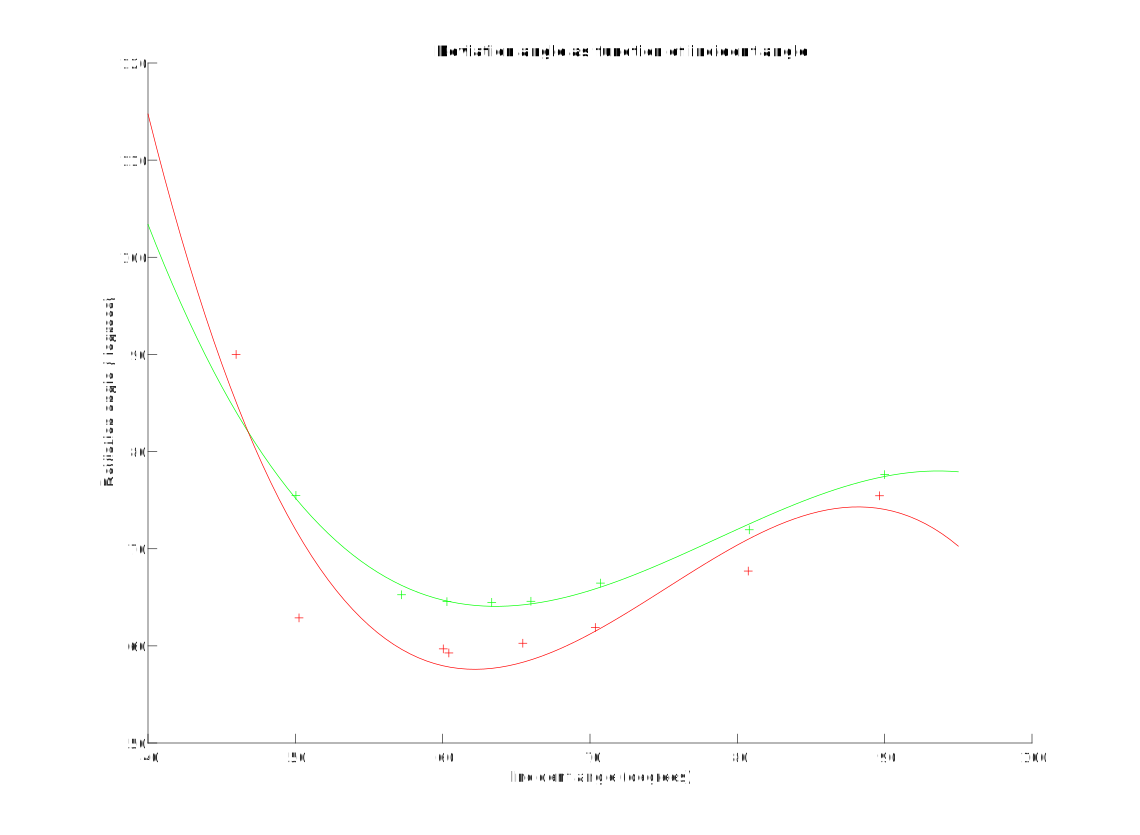
\includegraphics[width=\textwidth]{graph}
    \caption{Mätvärden plottade och tredjegradspolynom anpassade till mätvärdena. Gröna mätpunkter och kurvor motsvarar $\lambda_1$ och röda $\lambda_2$.}
    \label{fig: plot}
\end{figure}

\subsubsection{Rimlighetsbedömning av resultatet}
Vi skall diskutera om de givna avlänkningsvinklarna är rimliga under rådande förhållanden. För att göra denna rimlighetsbedömning skall
jag använda Snells brytningslag (ekvation \ref{eq:brytning}) och formeln för minsta avlänkning (ekvation \ref{eq:avlankning}). Med hjälp
av Snells brytningslag beräknar jag brytningsindex för de två våglängderna och prismats material. När vi känner till dessa kan vi med hjälp
av ekvation \ref{eq:avlankning} beräkna det som borde vara minsta avlänkningsvinkel. I GOT skapar jag ett rektangulärt glasblock och mäter
infalls- och brytningsvinkel. Jag antar att det infallande mediet är luft. För $\lambda_1=\SI{555}{\nano\meter}$ får vi $n_1 = 1.0, \alpha_1 = \ang{45}, \alpha_2 = \ang{23.42}$

\begin{equation}
    \begin{aligned}
        n_1 * sin(\alpha_1) = n_2 * sin(\alpha_2) \\
        n_2 = \frac{sin(\alpha_1)}{sin(\alpha_2)} \\
        n_2 = 1.779
    \end{aligned}
\end{equation}

Insättning i ekvation \ref{eq:avlankning} ger ett förväntat värde $\delta_1 = \ang{65.62}$ för ljus med våglängden 555 nm.

Mätningen med 700 nm ger en vinkel $\alpha_2 = \ang{23.91}$ ett brytningsindex $n_2 = 1.745$, vilket ger en minsta avlänkningsvinkel
$\delta = \ang{61.50}$. Jämfört med de uppmätta värdena verkar mätvärdena (och anpassningen) för $\lambda_1$ stämma bra,
men inte för $\lambda_2$. För $\lambda_2$ ser det sanna minimat ut att ligga kring \ang{60}, vilket överensstämmer bättre med det analytiska
resultatet. Anledningen till varför det inte kan stämma kan bero på det jag skall diskutera i nästa stycke.

\subsubsection{Rimlighetsbedömning av metoden}
Nu övergår diskussionen till huruvida metoden jag använde för att beräkna minsta avlänkningsvinkel är rimlig, om det finns något
att förbättra med den och i så fall, vad. Inledningsvis kan det nämnas att anledningen till att jag valde att anpassa just ett tredjegradspolynom
var att ett andragradspolynom gav ännu sämre anpassning, och ett fjärdegradspolynom gav ett orimligt utseende på kurvan. Självklart är inte sambandet
mellan infallsvinkel och anvlänkningsvinkel ett polynom, utan en komplicerad trigonometrisk funktion. Givetvis skulle man kunna anpassa
en sådan funktion till mätvärdena, men MATLAB har ingen sådan funktion inbyggd så det skulle vara alltför tidskrävande att göra det manuellt i detta fall.

Eftersom jag försöker representera en typ av samband med ett annat kommer det naturligtvis uppstå en felkälla där. En förbättring skulle
därför vara att analytiskt härleda detta trigonometriska samband och anpassa det till mätvärdena, istället för en godtycklig tredjegradskurva. Dessutom skulle
man i en framtida laboration kunna ta fler mätpunkter, speciellt kring området där minimat borde ligga, för att öka precisionen i resultatet.
I en optimal värld skulle man kunna skriva ett program som går igenom och tar mätvärden för exempelvis 100 eller 1000 värden mellan två angivna
infallsvinklar. Detta leder också in på vad som skulle kunna vara en felkälla till: nämligen precisionen hos mätningarna då de gjordes för hand
med hjälp av en digital linjal. En förbättring skulle alltså vara att modifiera GOT så att programmet också kan mäta avlänkningvinklar. Detta skulle
eliminera möjligheten för mänskligt fel just i det steget.

\subsection{Allmän diskussion kring svårigheter i laborationen}
För min del var det svårast att greppa hur mätningen av avlänkningsvinkeln skulle gå till. Först och främst måste man inse vilken vinkel som är
rätt, för att sedan lista ut hur man skall mäta den. Det tog mig några försök innan jag insåg vilken vinkel som var den rätta. Till en början 
satt jag också och funderade på om jag skulle mäta vinkeln för hand eller inte, men efter lite googlande hittade jag verktyget MB-Ruler.

Mitt tips till en framtida student är därför att vara rejält påläst kring prismafenomen innan man börjar laborationen, samt att använda sig av
verktyget MB-Ruler eller motsvarande för att mäta vinklar.

\section{Referenser}
\begingroup
\renewcommand{\section}[2]{}
\begin{thebibliography}{1}
    \bibliographystyle{plain}
    \bibitem{vl}
    Jönsson G. Våglära och Optik. Lund: Teach Support, 2018.
    \bibitem{wiki}
    Wikipedia. Beam divergence [Online]. \url{https://en.wikipedia.org/wiki/Beam_divergence} [2020-03-27]
    \bibitem{yt1}
    Mauritsson J. Kollimera [Online]. 2017. \url{https://youtu.be/G3TCW3y5oMc} [2020-03-27]
    \bibitem{yt2}
    Mauritsson J. Linjera [Online]. 2017. \url{https://youtu.be/8TzarQwkxPo} [2020-03-27]
    \bibitem{ins}
    Gustavsson D, Ahrling R. Appendix avbildningsfel i Optik 2020 [Online]. 2020. \url{https://canvas.education.lu.se/courses/3383/files/308598/download} [2020-03-27]
\end{thebibliography}
\endgroup

\pagebreak
\section{Appendix A - Kollimering och linjering}
\subsection{Kollimering}
Kollimering (från latin: collimare - kasta i rak riktning) innebär att man använder en konvex lins
för att parallellisera ljuset från en divergent ljuskälla. Detta görs genom att placera linsen
framför ljusstrålen, med fördel nära ljuskällan och justera avståndet till källan tills strålarna är parallella
på alla avstånd. En spegel kan användas så att ljuskälla och kollimeringspunkt hamnar bredvid varandra. Se figur \ref{fig:kollimering}.
Genom att placera linsen nära ljuskällan ser vi till att brännvidden blir oändlig \cite{yt1}.
\begin{figure}[h]
    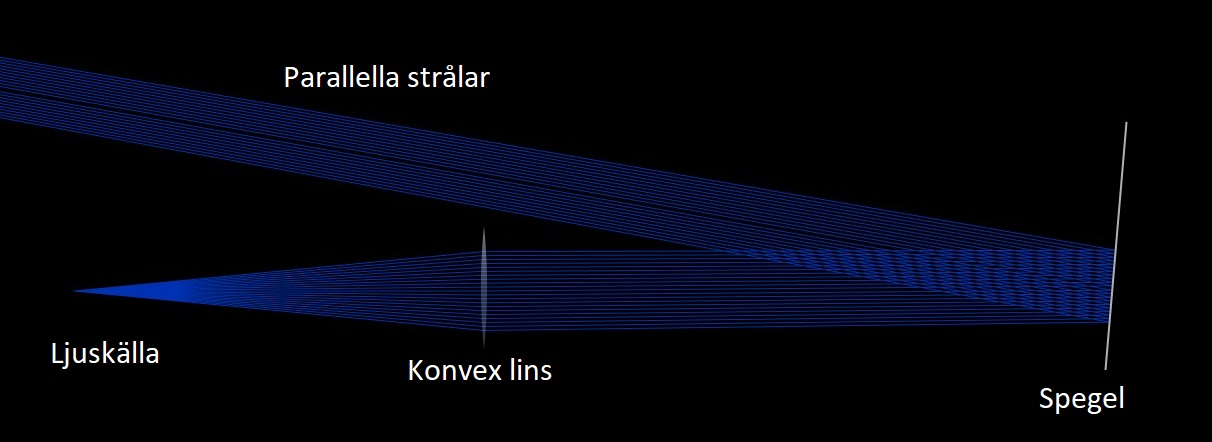
\includegraphics[width=\textwidth]{kollimera3.jpg}
    \caption{Kollimering av en divergent ljusstråle.}
    \label{fig:kollimering}
\end{figure}
\subsection{Linjering}
Att linjera lasern innebär att man tar en parallelliserad ljuskälla, exempelvis en laserstråle och ser till att det går igenom två bländare med rakast möjliga väg.
Detta görs genom att placera ut två speglar, en så nära den första bländaren som möjligt, och en så att ljusstrålen böjs ned mot den andra spegeln. Se figur \ref{fig:linjering}.
Sedan justeras spegel 1 i figuren så att ljuset passerar igenom första bländaren så centralt som möjligt. Sedan används spegel 2 för att se till att hela ljusstrålen passerar
genom den vänstra bländaren \cite{yt2}.
\begin{figure}[h]
    \centering
    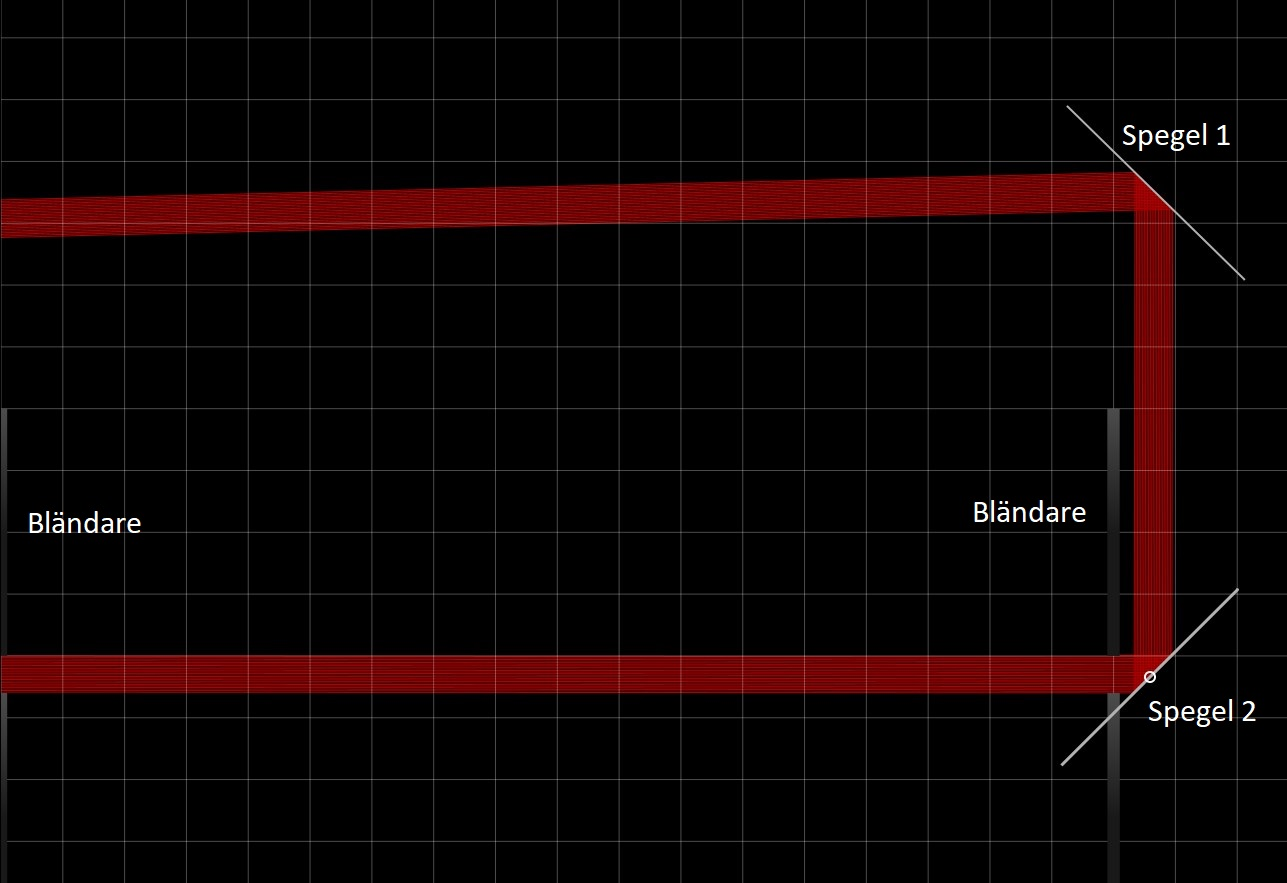
\includegraphics[width=0.6\textwidth]{linjera4.jpg}
    \caption{Kollimering av en divergent ljusstråle.}
    \label{fig:linjering}
\end{figure}
\pagebreak
\section{Övriga appendix}
Appendix B - MATLAB-kod från undersökningen av prismat. Återfinns på \url{https://raw.githubusercontent.com/zentabit/vaglara/master/laborationer/laboration1/measure.m}.

\end{document}
